% !TEX = root = ../../thesis.tex
\usetikzlibrary{shapes.geometric}
\usetikzlibrary{calc}
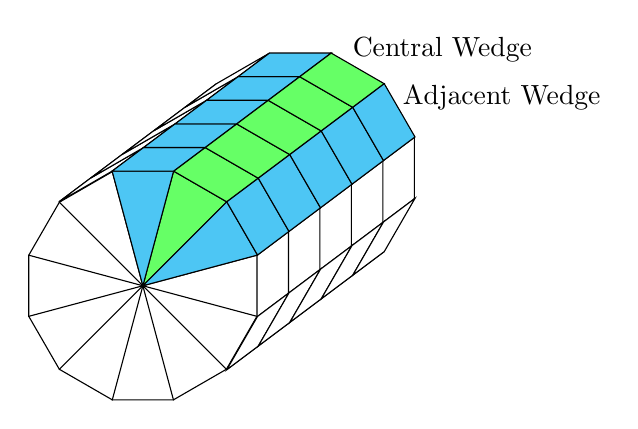
\begin{tikzpicture}

\def\dx{.4};
\def\dy{.3}
\def\r{3}
\def\c{1}
	
\node[draw, fill=white, regular polygon, regular polygon sides=12, minimum size=\r*\c cm] (w6) at (\dx*\c*5,\dy*\c*5){};
	
\node[draw, fill=white, regular polygon, regular polygon sides=12, minimum size=\r*\c cm] (w5) at (\dx*\c*4,\dy*\c*4){};

\node[draw, fill=white, regular polygon, regular polygon sides=12, minimum size=\r*\c cm] (w4) at (\dx*\c*3,\dy*\c*3){};

\node[draw, fill=white, regular polygon, regular polygon sides=12, minimum size=\r*\c cm] (w3) at (\dx*\c*2,\dy*\c*2){};

\node[draw, fill=white, regular polygon, regular polygon sides=12, minimum size=\r*\c cm] (w2) at (\dx*\c*1,\dy*\c*1){};

\node[draw, fill=white, regular polygon, regular polygon sides=12, minimum size=\r*\c cm] (w1) at (0,0){};

\foreach \i in {1,2,3,4,5,6,7,8,9,10,11,12}{
	\draw (0,0) -- (w1.corner \i);
}
\foreach \i in {1,2,3,9,10,11,12}{
	\draw (w1.corner \i) -- (w6.corner \i);
}


% Fixing perspective
\draw[fill=white] (w1.corner 9) -- (w2.corner 9) -- (w2.corner 10) -- (w1.corner 10) -- cycle;
\draw[fill=white] (w2.corner 9) -- (w3.corner 9) -- (w3.corner 10) -- (w2.corner 10) -- cycle;
\draw[fill=white] (w3.corner 9) -- (w4.corner 9) -- (w4.corner 10) -- (w3.corner 10) -- cycle;
\draw[fill=white] (w4.corner 9) -- (w5.corner 9) -- (w5.corner 10) -- (w4.corner 10) -- cycle;
\draw[fill=white] (w5.corner 9) -- (w6.corner 9) -- (w6.corner 10) -- (w5.corner 10) -- cycle;

\draw[fill=white] (w1.corner 2) -- (w2.corner 2) -- (w2.corner 3) -- (w1.corner 3) -- cycle;
\draw[fill=white] (w2.corner 2) -- (w3.corner 2) -- (w3.corner 3) -- (w2.corner 3) -- cycle;
\draw[fill=white] (w3.corner 2) -- (w4.corner 2) -- (w4.corner 3) -- (w3.corner 3) -- cycle;
\draw[fill=white] (w4.corner 2) -- (w5.corner 2) -- (w5.corner 3) -- (w4.corner 3) -- cycle;
\draw[fill=white] (w5.corner 2) -- (w6.corner 2) -- (w6.corner 3) -- (w5.corner 3) -- cycle;

% Central wedge
\draw[fill=green!60] (w1.corner 12) -- (w1.corner 1) -- (0,0) -- cycle;
\draw[fill=green!60] (w1.corner 12) -- (w2.corner 12) -- (w2.corner 1) -- (w1.corner 1) -- cycle;
\draw[fill=green!60] (w2.corner 12) -- (w3.corner 12) -- (w3.corner 1) -- (w2.corner 1) -- cycle;
\draw[fill=green!60] (w3.corner 12) -- (w4.corner 12) -- (w4.corner 1) -- (w3.corner 1) -- cycle;
\draw[fill=green!60] (w4.corner 12) -- (w5.corner 12) -- (w5.corner 1) -- (w4.corner 1) -- cycle;
\draw[fill=green!60] (w5.corner 12) -- (w6.corner 12) -- (w6.corner 1) -- (w5.corner 1) -- cycle;

% Adjacent wedge +1
\draw[fill=cyan!70] (w1.corner 11) -- (w1.corner 12) -- (0,0) -- cycle;
\draw[fill=cyan!70] (w1.corner 12) -- (w2.corner 12) -- (w2.corner 11) -- (w1.corner 11) -- cycle;
\draw[fill=cyan!70] (w2.corner 12) -- (w3.corner 12) -- (w3.corner 11) -- (w2.corner 11) -- cycle;
\draw[fill=cyan!70] (w3.corner 12) -- (w4.corner 12) -- (w4.corner 11) -- (w3.corner 11) -- cycle;
\draw[fill=cyan!70] (w4.corner 12) -- (w5.corner 12) -- (w5.corner 11) -- (w4.corner 11) -- cycle;
\draw[fill=cyan!70] (w5.corner 12) -- (w6.corner 12) -- (w6.corner 11) -- (w5.corner 11) -- cycle;
% Adjacent wedge -1

\draw[fill=cyan!70] (w1.corner 1) -- (w1.corner 2) -- (0,0) -- cycle;
\draw[fill=cyan!70] (w1.corner 2) -- (w2.corner 2) -- (w2.corner 1) -- (w1.corner 1) -- cycle;
\draw[fill=cyan!70] (w2.corner 2) -- (w3.corner 2) -- (w3.corner 1) -- (w2.corner 1) -- cycle;
\draw[fill=cyan!70] (w3.corner 2) -- (w4.corner 2) -- (w4.corner 1) -- (w3.corner 1) -- cycle;
\draw[fill=cyan!70] (w4.corner 2) -- (w5.corner 2) -- (w5.corner 1) -- (w4.corner 1) -- cycle;
\draw[fill=cyan!70] (w5.corner 2) -- (w6.corner 2) -- (w6.corner 1) -- (w5.corner 1) -- cycle;

%\node[text=green!60, label={right:Central Wedge}] at ($(w6.corner 12)!0.5!(w6.corner 1)$){};
\node[label={[right]:Central Wedge}, xshift=1ex, yshift=-.5ex] at (w6.corner 1){};
\node[label={[right]:Adjacent Wedge},xshift=0.75ex, yshift=-2ex] at (w6.corner 12){};

\end{tikzpicture}
